% Chapter 2

\chapter{Randomized classification} % Main chapter title

\label{Chapter2} % For referencing the chapter elsewhere, use \ref{Chapter1} 

As we foreshadowed in the introduction, randomized classification is
also one of the three methods we consider for evaluating
representations.  Yet, two other applications of randomized
classification are (i) for providing a formalism for evaluting
\emph{recognition systems}, and (ii) for studying generalizability of
certain classification-based experiments.  The application of
recognition systems provides the most intuitive way of understanding
the randomized classification task; therefore, in this chapter, we
begin with a discussion in section \ref{sec:recog_tasks} of
recognition tasks, and within this context, motivate the definition of
a randomized classification task in section \ref{sec:rc_motivation}.
We propose to use the randomized classification task to model the
problem of recognition, and to evalaute performance via the
\emph{average accuracy}.  Next, to put our ideas into practice, we
need ways to estimate the average accuracy from data, which we address
in \ref{sec:estimation_average_accuracy}.

Meanwhile, the problem of generalizing classification experiments
provides a natural motivation for studying the variance of
classification accuracy within a randomized classification task, which
we cover in section \ref{sec:average_bayes_accuracy}.  Meanwhile,
another one of the methods we consider--the identification risk, is
closely connected with the randomized classification task.  We discuss
how our results in \ref{sec:average_bayes_accuracy} can also be
applied to the identification case.

\section{Recognition tasks}\label{sec:recog_tasks}

Human brains have a remarkable ability to recognize objects, faces,
spoken syllables and words, and written symbols or words, and this
recognition ability is essential for everyday life.  While researchers
in artificial intelligence have attempted to meet human benchmarks for
these classical recognition tasks for the last X decades, only very
recent advances in machine learning, such as deep neural networks,
have allowed algorithmic recognition algorithms to approach or exceed
human performance [CITE].

Within the statistics and machine learning literature, the usual
formalism for studying a recognition task is to pose it as a
\emph{multi-class classification} problem.  One delineates a finite
set of distinct entities which are to be recognized and distinguished,
which is the \emph{label set} $\mathcal{Y}$.  The input data is
assumed to take the form of a finite-dimensional real \emph{feature
  vector} $X \in \mathbb{R}^p$.  Each input instance is associated
with exactly one true label $Y \in \mathcal{Y}$.  The solution to the
classification problem takes the form of an algorithmically
implemented \emph{classification rule} $h$ that maps vectors $X$ to
predicted labels $\hat{Y} \in \mathcal{Y}$.  The classification rule
can be constructed in a data-dependent way: that is, one collects a
number of labelled \emph{training observations} $(X_1, Y_1)$ which is
used to inform the construction of the classification rule $h$.  The
quality of the classification rule $h$ is measured by \emph{generalization accuracy}
\[
\text{GA}(h) = \Pr[h(X) = Y],
\]
where the probability is defined with reference to the unknown
population joint distribution of $(X, Y)$.  

However, a limitation of the usual multi-class classification
framework for studying recognition problems is the assumption that the
label set $\mathcal{Y}$ is finite and known in advance.  When
considering human recognition capabilities, it is clear that this is
not the case.  Our ability to recognize faces is not limited to some
pre-defined, fixed set of faces; same with our ability to recognize
objects in the environment.  Humans learn to recognize novel faces and
objects on a daily basis.  And, if artificial intelligence is to fully
match the human capability for recognition, it must also possess the
ability to add new categories of entities to its label set over time;
however, at present, there currently exists a void in the machine
learning literature on the subject of the online learning of new
classes in the data [CITE].

The central theme of this thesis is the study of \emph{randomized
  classification}, which can be motivated as an extension of the
classical multi-class classification framework to accommodate the
possibility of growing or infinite label sets $\mathcal{Y}$. The basic
approach taken is to assume an infinite or even continuous label space
$\mathcal{Y}$, and then to study the problem of classification on
finite label sets $S$ which are randomly sampled from $\mathcal{Y}.$
This, therefore defines a \emph{randomized classification} problem
where the label set is finite but may vary from instance to instance.
One can then proceed to answer questions about the variability of the
performance due to randomness in the labels, or how performance
changes depending on the size of the random label set.

\section{Randomized classification}\label{sec:rc_motivation}

\subsection{Motivation}
The formalism of classification is inadequate for studying
many practical questions related to the generalizability of the facial
recognition system.  We can define a population risk (also called
generalization error) for the classification rule, and make inferences
about the population risk based on the test performance.  However, the
population risk and associated inferences apply only to the particular
collection of individuals $\{y^{(1)},\hdots, y^{(k)}\}$.  If we were
to add a new individual $y^{(k+1)}$ to the dataset, for instance, when
photographs are uploaded on Facebook containing a new user, this
defines a totally new classification problem because the expanded set
of labels $\{y^{(1)},\hdots, y^{(k+1)}\}$ defines a different response
space than the old set of labels $\{y^{(1)},\hdots, y^{(k)}\}$.  Yet,
these two classification problems are clearly linked.  To take another
example, a client might want to run the facial recognition system on
their own database of individuals.  In this case, there might be no
overlap between the first set of labels (the people in my database)
and the second set of labels (the people in the client's database.)
And yet, the client might still expect the performance of the system
on our database to be informative of how well it will do on the second
set of labels!

The question of how to link performance between two different but
related classification tasks is an active area of research, known as
\emph{transfer learning}.  But while the two examples we just listed
might be considered as examples of transfer learning problems, the
current literature on transfer learning, as far as we know, does not
study the problem of \emph{mutating label sets}.  Therefore, to
address this new class of questions about the generalizability of the
recognition system, we need to formalize our notions of (a) what
constitutes a `recognition system' which can be applied to different
classification problems, and (b) what assumptions about the problem,
and what assumptions about the classifiers used, allow one to infer
performance in one classification problem based on performance in
another classification problem.

\subsection{Setup}
By `recognition system,' we really mean a \emph{learning algorithm}
$\Lambda$ which can take training data as input, and produce a
classification rule for recognizing faces.  While a classification
rule is bound to a specific label set, a learning algorithm can be
applied to datasets with arbitrary label sets, and be continually
updated as new labels are added to the label set.  To `update' a
facial recognition system with new data means to apply the learning
algorithm to the updated database.

Now we can formalize what it means to generalize performance from one
problem to another.  A \emph{classification problem} $P$ is specified
by a label set $\mathcal{Y}$, a predictor space $\mathcal{X}$, a joint
distribution $G$ on $\mathcal{X} \times \mathcal{Y}$, and a
\emph{sampling scheme} $S$ for obtaining training data (for example,
to obtain $n$ observations from $G$ i.i.d.).  The sampling scheme is
needed because we cannot say much about how the learning algorithm
will perform unless we know how much training data it is going to
have.  The generalization accuracy (GA) of the algorithm $\Lambda$ on the
classification problem $P = (\mathcal{Y}, \mathcal{X}, G, S)$ is
defined as the expected risk of the resulting classification rule $h$,
\[
\text{GA}_P(\Lambda) = \E[\text{GA}(h)]
\]
where $h$ is produced by applying $\Lambda$ to the training data,
sampled by $S$.  The expectation is taken over the randomness in the
generation of the training data.

At this point we have defined an extremely general transfer learning
problem: given two different classification problems $P_1 =
(\mathcal{Y}_1, \mathcal{X}_1, G_1, S_1)$ and $P_2 = (\mathcal{Y}_2,
\mathcal{X}_2, G_2, S_2)$, what can we say about the relationship
between $\text{GA}_{P_1}(\Lambda)$ and $\text{GA}_{P_2}(\Lambda)$?
Not much, unless we make many more assumptions about how $P_1$ and
$P_2$ are linked.

The basic approach we will take is to assume that both $P_1$ and $P_2$
have been generated randomly via a common mechanism.  In the original
motivating context of facial recognition, this is to say that two
different label sets $\mathcal{Y}_1$ and $\mathcal{Y}_2$ are linked
because they both belong to a common population of labels
$\mathcal{Y}$, i.e., the population of all possible humans, and to
further assume that both have been \emph{sampled}, in the same manner,
from $\mathcal{Y}$.

The study of how to make inferences about the risk in $P_2$ given
information about the performance achieved in $P_1$, granted a set of
assumptions on how $P_1$ and $P_2$ have been randomly generated (and
are thereby linked through shared randomization mechanisms) forms the
basis of the subject of \emph{randomized classification}.

As we noted in the introduction, the problem of randomized
classification has a close ancestor in the study of \emph{random code
  models} in information theory.  There, the problem is to understand
the \emph{decoding performance} (the analogue to risk) of a
encoding/decoding system $P$ which has a randomized code space
$\mathcal{Y}$.  Where random code models have a random codebook which
is a sample over a distribution of all possible codes, randomized
classification problems have a random label set that is a sample of a
larger label space.  However, the results we obtain for randomized
classification are more general in nature than the existing results
availible for random code models, because work on random codes is
generally limited to asymptotic settings, whereas we obtain finite-$k$
results, and because random code models assume a specific
product-distribution structure on $(X, Y)$ which is not appropriate
for classification problems.

\subsection{Assumptions}

The randomized classification model we study has the following
features.  We assume that there exists an infinite (or even
continuous) label space $\mathcal{Y}$ and a response space
$\mathcal{X} \in \mathbb{R}^p$.  For each label $y \in \mathcal{Y}$,
there exists a distribution of features $F_y$.  Furthermore, there
exists a prior distribution $\pi$ on $\mathcal{Y}$.

A random classification task $P$ can be generated as follows.  The
label set $\mathcal{S} = \{Y^{(1)},\hdots, Y^{(k)}\}$ is generated by
drawing labels $Y^{(1)},\hdots, Y^{(k)}$ i.i.d. from $\pi$.  The joint
distribution $G$ of pairs $(X, Y)$ is uniquely specified by the two
conditions that (i) the marginal distribution of $Y$ is uniform over
$\mathcal{S}$, and (ii) the conditional distribution of $X$ given
$Y=Y^{(i)}$ is $F_{Y^{(i)}}$.  We sample both a training set and a
test set.  The training set is obtained by sampling $r_1$ observations
$X_{j, train}^{(i)}$ i.i.d. from $F_{Y^{(i)}}$ for $j = 1,\hdots,
r_1$.  The test set is likewise obtained by sampling $r_2$
observations $X_j^{(i)}$ i.i.d. from $F_{Y^{(i)}}$ for $j = 1,\hdots,
r_2$.  For notational convenience, we represent the training set as
the set of empirical distributions $\{\hat{F}_{Y^{(i)}}\}_{i=1}^k$
where
\[
\hat{F}_{Y^{(i)}} = \frac{1}{r_1} \sum_{j=1}^{r_1} \delta_{X^{(i)}_{j, train}}.
\]
Figure \ref{fig:training_set} illustrates the sampling scheme for
generating the training set.

\begin{figure}[h]
\centering
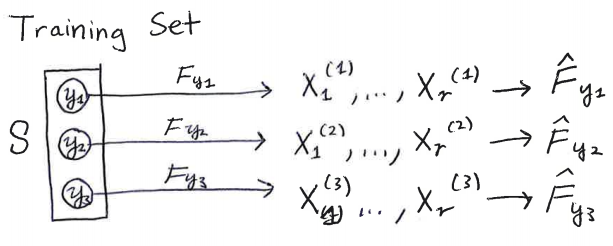
\includegraphics[scale = 0.4]{../extrapolation_figures/training_set.png}
\caption{Training set}\label{fig:training_set}
\end{figure}

Our analysis will also rely on a property of the classifier. We do not
want the classifier to rely too strongly on complicated interactions
between the labels in the set. We therefore propose the following
property of marginal separability for classification models:

\begin{definition}
\begin{enumerate}
\item The classification rule $h$ is called a \emph{marginal rule} if 
\[
h(x) = \text{argmax}_{y \in \mathcal{S}} m_y(x),
\]
where the function $m_y$ maps $\mathcal{X}$ to $\mathbb{R}$. 
\item Define a marginal model $\mathcal{M}$ as a mapping from empirical distributions
to margin functions,
\[
\mathcal{M}(\hat{F}_y) = m_y(x).
\]
\item A classifier that produces marginal classification rules
\[
h(x) = \text{argmax}_{y \in \mathcal{S}} m_y(x),
\]
by use of a marginal model, i.e. such that
$m_y=\mathcal{M}(\hat{F}_y)$ for some marginal model $\mathcal{M}$,
is called a \emph{marginal classifier}.
\end{enumerate}
\end{definition}
In words, a marginal classification rule produces a \emph{margin}, or
score, for each label, and chooses the label with the highest
margin. The marginal model converts empirical distributions
$\hat{F_y}$ over $\mathcal{X}$ into the margin function
$m_y$.  The \emph{marginal} property allows us to prove strong results
about the accuracy of the classifier under i.i.d. sampling assumptions.

\textbf{Comments:}
\begin{enumerate}
\item The marginal model includes several popular classifiers.
A primary example for a marginal model is the estimated Bayes
classifier. Let $\hat{f_y}$ be a density estimate obtained from the
empirical distribution $\hat{F_y}$. Then, we can use the estimated
densities of each class to produce the margin functions:
\[ m^{EB}_y(x) = \log(\hat{f_{y}}(x)).\]
The resulting empirical approximation for the Bayes classifier
(further assuming a uniform prior $\pi$) would be
\[ f^{EB}(x) = \text{argmax}_{y \in \mathcal{S}}(m^{EB}_y(x)).\]
\item Both the Quadratic Discriminant Analysis and the naive Bayes classifiers can be seen as specific instances of an estimated Bayes classifier
\footnote{QDA is the special case of the estimated Bayes classifier when $\hat{f_y}$ is obtained as
the multivariate Gaussian density with mean and covariance parameters estimated from the data.
Naive Bayes is the estimated Bayes classifier when $\hat{f_y}$ is obtained as the product of estimated componentwise marginal distributions
of $p(x_i|y)$}. 
For QDA, the margin function is
given by
\[
m_y^{QDA}(x) = -(x - \mu(\hat{F}_y))^T \Sigma(\hat{F}_y)^{-1} (x-\mu(\hat{F}_y)) - \log\det(\Sigma(\hat{F}_y)),
\]
where $\mu(F) = \int y dF(y)$ and $\Sigma(F) = \int (y-\mu(F))(y-\mu(F))^T dF(y)$.
In Naive Bayes, the margin function is
\[
m^{NB}_y(x) = \sum_{i=1}^n \log \hat{f}_{y, i}(x),
\]
where $\hat{f}_{y, i}$ is a density estimate for the $i$-th component of
$\hat{F}_y$.
\item There are also many classifiers which do not satisfy the marginal property, such as multinomial logistic regression,
multilayer neural networks, decision trees, and k-nearest neighbors.
\end{enumerate}

The operation of a marginal classifier is illustrated in figure
\ref{fig:classification_rule}.  Since a marginal classifier is
specified entirely by its marginal model $\mathcal{M}$, we will take
the notational convention of referring to a marginal classifier as
$\mathcal{M}$.

\begin{figure}[h]
\centering
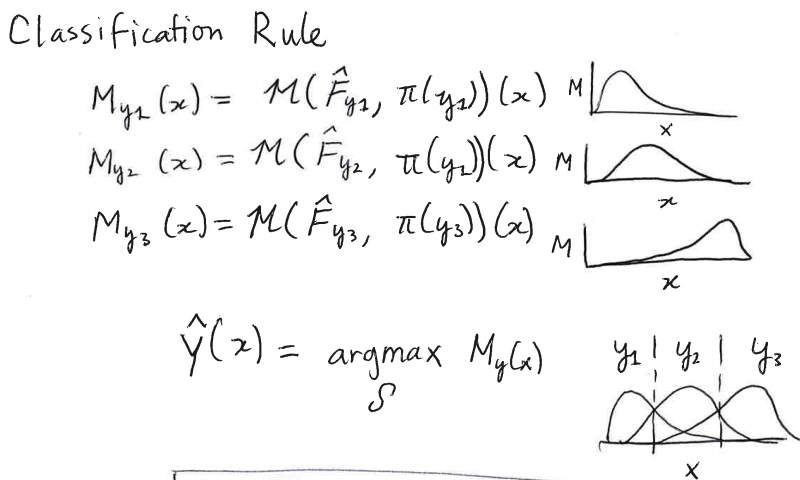
\includegraphics[scale = 0.4]{../extrapolation_figures/classification_rule.png}
\caption{Classification rule}\label{fig:classification_rule}
\end{figure}

We would like to identify the sources of randomness in evaluating a
classifier.  First, there is the specific choice of $k$ classes for
the label set.   Second, there is randomness in training the classifier
for these classes, which comes from the use of a finite training
set. Third, there is the randomness in the estimated risk when
testing the classifier on a test set.

If we \emph{fix} a particular realization of the random label set
$\mathcal{S} = \{y^{(1)}, \hdots, y^{(k)}\}$ as well as the training
set $\{\hat{F}_{y^{(i)}}\}_{i=1}^k$, then the classifier $h(x)$ is
fixed, and only the third source of randomness (in test risk) applies.
However, the true generalization accuracy of the classifier is deterministic:
\begin{align*}
\text{GA}(h) &= \Pr[Y = h(X)|Y \sim \text{Unif}(\mathcal{S}),
  \mathcal{S}, \{\hat{F}_{y^{(i)}}\}_{i=1}^k] 
\\&= \frac{1}{k}
\sum_{i=1}^k \Pr[m_{y^{(i)}}(x) = \max_j m_{y^{(j)}}(x)|X \sim
  F_{y^{(i)}}, \mathcal{S}, \{\hat{F}_{y^{(i)}}\}_{i=1}^k].  
\\&= \frac{1}{k}
\sum_{i=1}^k I(m_{y^{(i)}}(x) = \max_j m_{y^{(j)}}(x)) dF_{y^{(i)}}(x).
\end{align*}

If we \emph{fix} a particular realization of the random label set
$\mathcal{S} = \{y^{(1)}, \hdots, y^{(k)}\}$, then we can define the
(generalization) accuracy specific to that label set.  However, the
training data $\{\hat{F}_{y^{(i)}}\}_{i=1}^k$ will be random.  Let us
denote the \emph{distribution} of the empirical distribution
$\hat{F}_y$ constructed from sample size $r$ as $\Pi_{y, r}$.  The
accuracy of the classifier $\mathcal{M}$ on label set $\mathcal{S}$ is
given by
\begin{align*}
\text{GA}_{\mathcal{S}}(\mathcal{M}) &= \Pr[Y = h(X)|Y \sim
  \text{Unif}(\mathcal{S}), \hat{F}_{y^{(i)}} \sim \Pi_{y^{(i)}, r_1}] \\&= \frac{1}{k} \sum_{i=1}^k \int
I(\mathcal{M}(\hat{F}_{y^{(i)}})(x) = \max_j
\mathcal{M}(\hat{F}_{y^{(j)}})) dF_{y^{(i)}}(x) \prod_{\ell=1}^k
d\Pi_{y^{(\ell)}, r_1}(\hat{F}_{y^{(\ell)}}).
\end{align*}
The calculation of the accuracy (for fixed label set $\mathcal{S}$) is
illustrated in figure \ref{fig:risk}.

\begin{figure}[h]
\centering
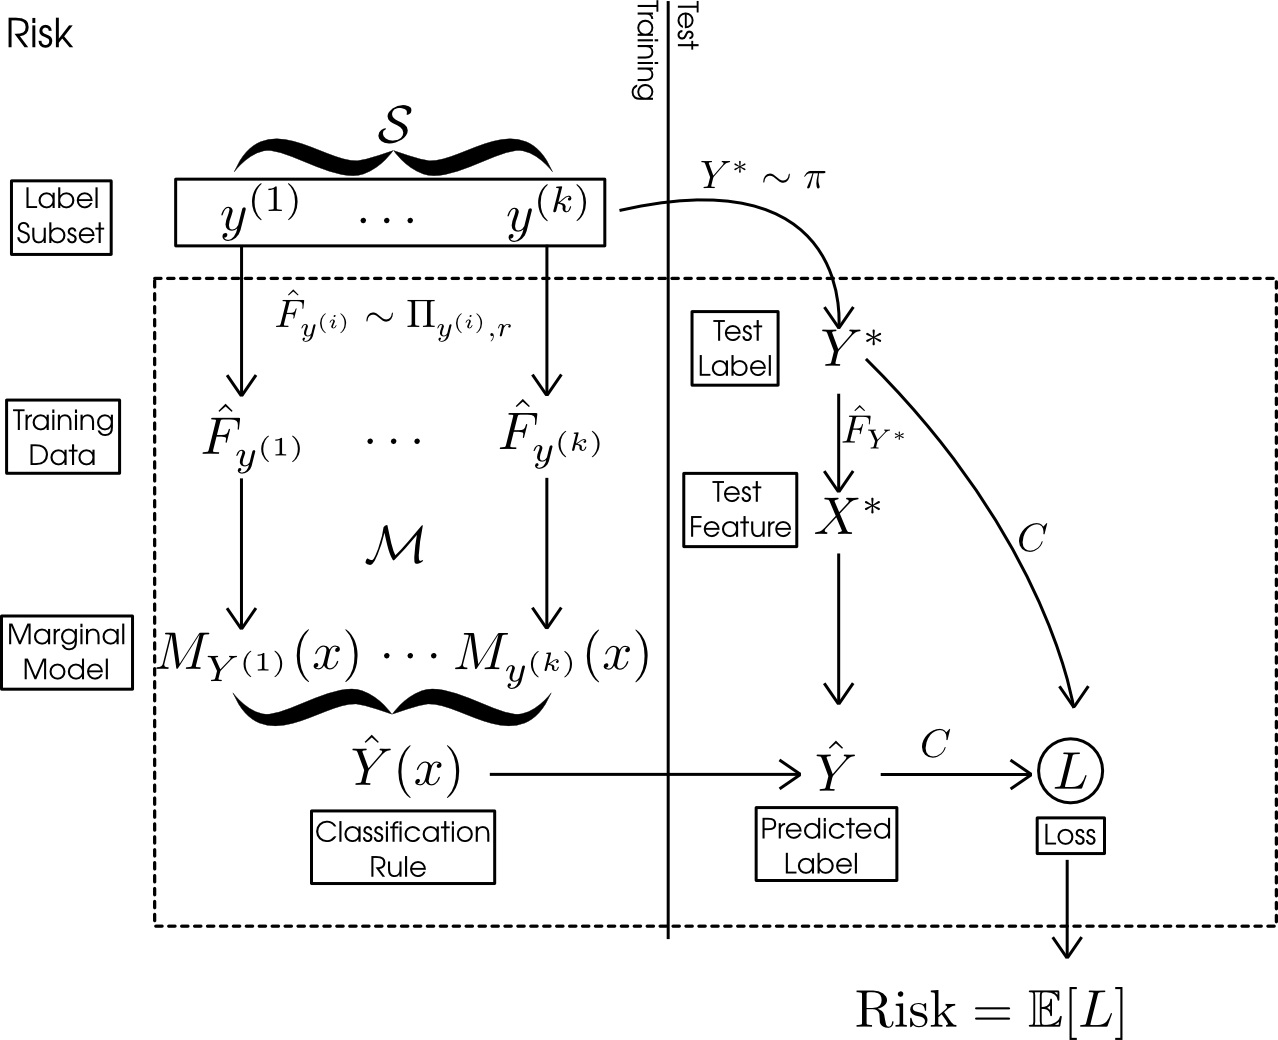
\includegraphics[scale = 0.3]{../extrapolation_figures/risk.png}
\caption{Generalization accuracy [NOTE: risk is 1-accuracy, figure to be fixed later!]}\label{fig:risk}
\end{figure}

Finally, suppose we do not fix any of the random quantities in the
classification task $P$, and merely specify $k$, the number of
classes, and $r_1$, the number of repeats in the training set.  
Then the $k$-class, $r$-repeat \emph{average generalization accuracy} of
a marginal classifier $\mathcal{M}$ is defined as
\begin{align*}
\text{AGA}_{k,r_1}(\mathcal{M}) &= \E[\text{FA}_{\mathcal{S}}(\mathcal{M})|Y^{(1)}, \hdots, Y^{(k)} \sim \pi]
\\&= \frac{1}{k} \sum_{i=1}^k \int
I(\mathcal{M}(\hat{F}_{y^{(i)}})(x) = \max_j
\mathcal{M}(\hat{F}_{y^{(j)}})) dF_{y^{(i)}}(x) \prod_{\ell=1}^k
d\Pi_{y^{(\ell)}, r_1}(\hat{F}_{y^{(\ell)}}) d\pi(y^{(\ell)}).
\end{align*}
The definition of average generalization accuracy is illustrated in Figure \ref{fig:average_risk}.

\begin{figure}[h]
\centering
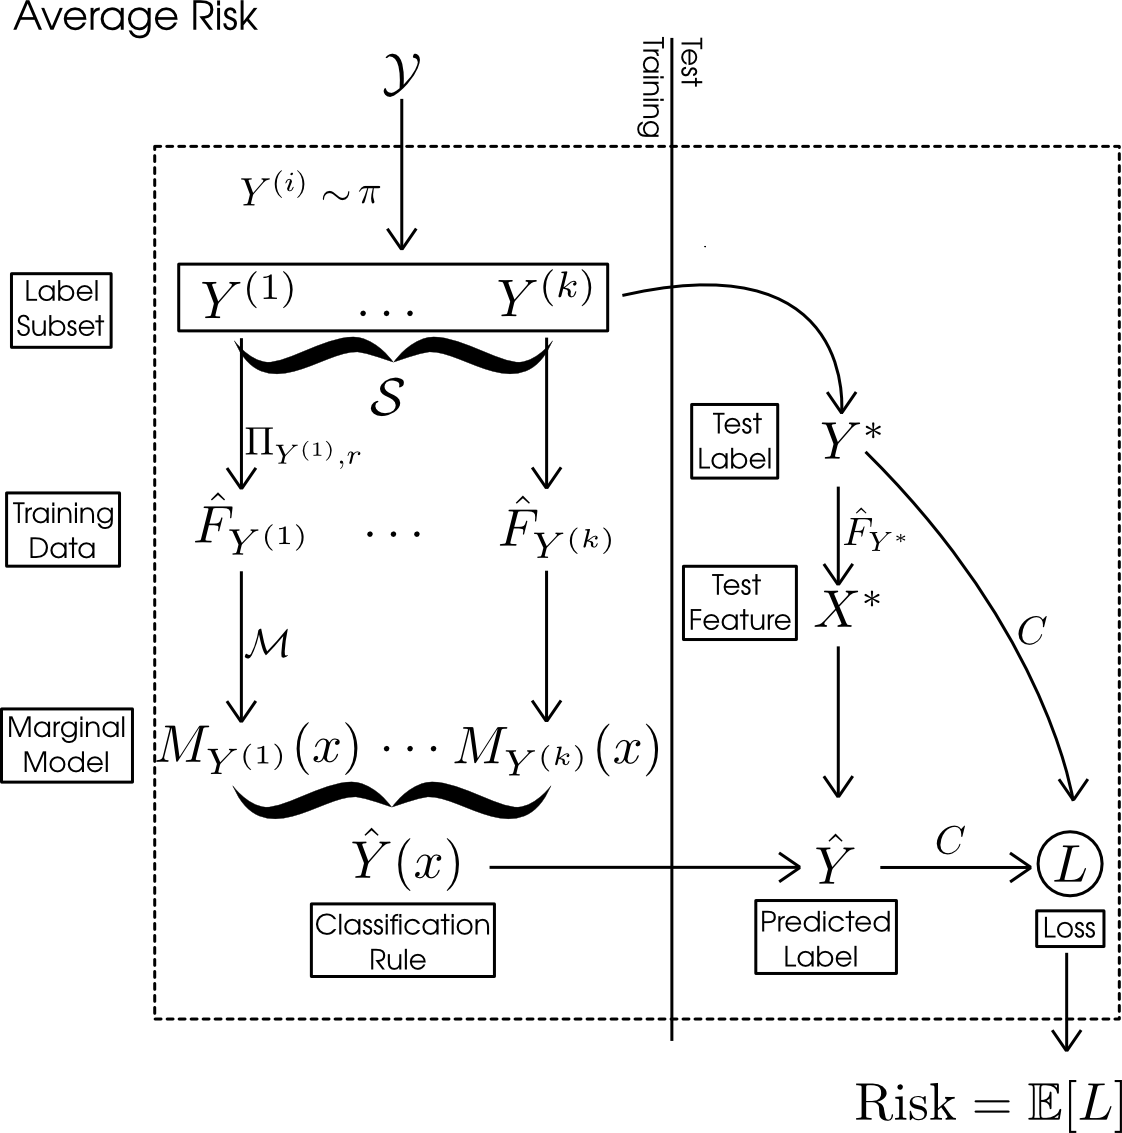
\includegraphics[scale = 0.3]{../extrapolation_figures/average_risk.png}
\caption{Average generalization accuracy [NOTE: risk is 1-accuracy, figure to be fixed later!]}\label{fig:average_risk}
\end{figure}

Having defined the average (generalization) accuracy for the randomized classification
task, we begin to develop the theory of how to \emph{estimate} the
average accuracy in the next section.

\section{Estimation of average accuracy}\label{sec:estimation_average_accuracy}

Suppose we have training and test data for a classification task $P_1$
with $k_1$ classes, $r_1$-repeat training data and $r_2$-repeat test
data.  That is, we have label set $\mathcal{S}_1 =
\{y^{(i)}\}_{i=1}^{k_1}$, as well as training sample $\hat{F}_{y^{(i)}}$
and test sample $(x_1^{(i)},\hdots, x_{r_2}^{(i)})$ for $i =
1,\hdots, k_1$.  How can we estimate the $k, r$-average accuracy of a
marginal classifier $\mathcal{M}$ for arbitrary $k$ and $r$?

Let us start with the case $k = k_1$ and $r = r_1$.  Then the answer
is simple: construct the classification rule $h$ using marginal model
$\mathcal{M}$ from the training data.  Then the test accuracy of $h$ is an
unbiased estimator of $\text{AGA}_{k,r}$.

This follows from definition.  Observe that $\text{AGA}_{k_1,r_1}$ is
the expected prediction risk for the classification rule $h$ for a
randomized classification problem $P$ with $k_1$ classes and
$r_1$-repeat training data.  Of course, the classification task $P_1$
that we have been given is a random drawn from the dersired
distribution of random classification problems.  Therefore, the
prediction risk of $h$ constructed from $P_1$ is unbiased for
$\text{AGA}_{k_1, r_1}$, and since test accuracy is unbiased for
generalization accuracy, it follows that the test accuracy of $h$ is
an unbiased estimator of $\text{AGA}_{k,r}$, as we claimed.

In following sections, we consider more complicated cases where $k_1
\neq k$.  However, before proceeding, let us first review the
procedure for computing the test accuracy.

For any given test observation $x_j^{(i)}$, we obtain the predicted
label $\hat{y}_j^{(i)}$ by computing the margin for each class,
\[
M_{i,j,\ell} = \mathcal{M}(\hat{F}_{y^{(\ell)}})(x_j^{(i)}) =  m_{y^{(\ell)}}(x_i^{(j)}),
\]
for $\ell = 1,\hdots, k_1$,
and by finding the class with the highest margin $M_{i, j, \ell}$,
\[
\hat{y}_j^{(i)} = y_{\argmax_\ell M_{i, j, \ell}}.
\]
The test accuracy is the fraction of correct classification over test observations,
\begin{equation}
\text{TA} = \frac{1}{r_2k} \sum_{i=1}^k \sum_{j=1}^{r_2} I(\hat{y}_j^{(i)} = y^{(i)}).
\end{equation}
For each test observation, define the ranks of the margins by
\[
R_{i,j,\ell} = \sum_{m \neq \ell} I\{M_{i,j,\ell} \geq M_{i, j, m}\}.
\]
Therefore, $\hat{y}_j^{(i)}$ is equal to $\ell$ if and only if $R_{i,j,\ell} = k$.
Thus, an equivalent expression for test accuracy is
\begin{equation}\label{eq:test_risk}
\text{TA} = \frac{1}{r_2 k_1} \sum_{i=1}^{k_1} \sum_{j=1}^{r_2} I\{R_{iji} = k_1\}.
\end{equation}

\subsection{Subsampling method}

Next, let us consider the case where $k < k_1$ and $r=r_1$.  Define a
classification problem $P_2$ with label set $\mathcal{S}_2$ obtained
by sampling $k$ labels uniformly without replacement from
$\mathcal{S}_1$.  Let the training and test data for $P_2$ be obtained
by taking the training data and test data from $P_1$ belonging to
labels in $\mathcal{S}_1$.  It follows that $P_2$ is a randomized
classification task with $k$ labels, $r_1$-repeat training data and
$r_2$-repeat test data.  Therefore, by the previous argument, the test
accuracy for a classification rule $h$ constructed using the training data
in $P_2$ provides an unbiased estimate of $\text{AGA}_{k, r_1}$.

However, we can get a much better unbiased estimate of
$\text{AGA}_{k, r_1}$ by averaging over the randomization of
$\mathcal{S}_2$.  Na\"{i}vely, this requires us to train and evaluate
${k_1}\choose{k}$ classification rules.  However, due to the special
structure of marginal classifiers, we do the computation in the same
order of computation as evaluating a single classification rule
(assuming that the computational bottleneck is in training the
classifier.)

This is because the rank $R_{iji}$ of the correct label, $i$, for the
$x_j^{(i)}$ allows us to determine how many subsets $\mathcal{S}_2$
will result in a correct classification.  For example $x_j^{(i)}$,
there are $R_{iji} - 1$ labels with a lower margin than the correct
lable $i$.  Therefore, as long as one of the classes in
$\mathcal{S}_2$ is $i$, and the other $k-1$ labels are from the set of
$R_{iji}-1$ labels with lower margin than $i$, the classification of
$x_j^{(i)}$ will be correct.  This implies that there are
${R_{iji}-1}\choose{k-1}$ such subsets $\mathcal{S}_2$ where
$x_j^{(i)}$ is classified correctly, and therefore

\begin{equation}\label{eq:avtestrisk}
\text{AverageTA}_{k, r_1} = \frac{1}{{{k_1}\choose{k}}}\frac{1}{r_2 k} \sum_{i=1}^{k_1} \sum_{j=1}^{r_2} {{R_{iji}-1}\choose{k-1}}.
\end{equation}

\subsection{Extrapolation}

A much more challenging case is when $k_2 > k_1$: that is, we want to
predict the performance of the classification model in a setting with
more labels than we currently see in the training set.  This is the
subject of Chapter 3.

\subsection{Variance bounds}

By now we have developed unbiased estimators for average generalization accuracy in the
special case $k \leq k_1$, and the following chapter will present
methods for the more difficult case $k > k_1$.  However, to get useful
inference statements, we also have to understand the variance of these
estimators.  For the large part, this is still work-in-progress.
However, some first steps towards addressing this problem are
described in the next section.

\section{Reproducibility and Average Bayes accuracy}\label{sec:average_bayes_accuracy}

\subsection{Motivation}

In task fMRI experiments, one typically obtains data of the form
$(\vec{x}_i, y_i)$, where $\vec{x}_i$ are activity patterns obtained
from the fMRI scan for a region of interest, and $y_i$ are categories
for tasks.  The labels $y_i$ are limited to a discrete set
$\{y^{(1)},\hdots, y^{(k)}\}$.  Data-splitting is used to obtain an
estimated generalization accuracy $\hat{\text{GA}}$ for predicting $y$
from $\vec{x}$.  The generalization accuracy is then interpreted as
evidence for the specialization of that region of interest for the
task at hand: a high accuracy suggests that the region is specialized
for the task, while a low accuracy suggests that the region is not
specialized for the task.

However, a limitation of this approach is the poor reproducibility of
the estimated generalization accuracy $\hat{\text{GA}}$.  Besides the
dependence of $\hat{\text{GA}}$ on the particular subject
participating in the experiment, the amount of training data, and the
classifier used, but the classification task is often inconsistent
from lab to lab.  That is because the task exemplars--that is, the set
of labels $\{y^{(i)}\}_{i=1}^k$, may be arbitrarily specified, and
therefore even ignoring the effect of subject, amount of training
data, and classifier, the estimation target $\text{GA}$ depends on
an arbitrary choice of exemplars.

On the other hand, fixing in advance the set of exemplars
$\{y^{(i)}\}_{i=1}^k$ is also not a satisfactory solution, since the
objective of the experiment is to understand the general relation
between the task and the region of interest, and not the relationship
between a particular set of task exemplars $\{y^{(i)}\}_{i=1}^k$ and
the region of interest.

Randomized classification provides a solution for addressing both the
variability in estimation target and generalization to the population,
as long as one can justify the assumption that the labels
$\{y^{(i)}\}_{i=1}^k$ are a random sample from some population of task
exemplars $\pi$.  While the generalization accuracy $\text{GA}$ for
any particular, fixed set of exemplars is \emph{not} a population
parameter, the average generalization accuracy $\text{AGA}$ \emph{is}
defined with reference to a population, albeit also dependent on a
specific classifier and sampling scheme.  Meanwhile, the limitations
on reproducibility due to differing choices of labels sets can be
understood based on the variability properties of $\text{GA}$.

However, one can argue that randomized classification does not go far
enough to ensure generalizability of results, because $\text{AGA}$
still depends on the sampling scheme (the amount of training data) and
the choice of classifier, which are both arbitrary experimental
choices.  Therefore, our proposal is to treat the average \emph{Bayes}
accuracy as the estimation target of interest.  The average Bayes
accuracy is defined independently of the classifier and sampling
scheme, and we will develop tools for inferring probabilistic lower
bounds (lower confidence bounds) of the average Bayes accuracy in this
section.

\subsection{Setup}

%% todo: switch notations in this section

Define the generalization accuracy of a classification rule $f$ as the complement
of its risk (under zero-one loss),
\[
\text{GA}(f) = \Pr[Y = f(X)].
\]

The generalization accuracy of any classification rule is
upper-bounded by the accuracy of the optimal classification rule, or
\emph{Bayes rule.}  That is, one can define the \emph{Bayes accuracy}
as
\[
\text{BA} = \sup_f \text{GA}(f).
\]
And due to Bayes' theorem, the optimal classification rule $f^*$ which
achieves the Bayes accuracy can be given explicitly: it is the maximum a
posteriori (MAP) rule
\[
f^*(x) = \argmax_{i=1}^k\ p(x|y^{(i)}).
\]
Of course, it is not possible to construct this rule in practice since
the joint distribution is unknown.  Instead, a reasonable approach is
to try a variety of classifiers, producing rules $f_1,\hdots, f_m$,
and taking the best generalization accuracy as an estimate of the Bayes
accuracy. 

Now consider a randomized classification task where the labels
$\{Y^{(1)},\hdots, Y^{(k)}\}$ are drawn iid from a population $\pi$,
and where the observations $X$ for label $Y$ are drawn from the
conditional distribution $F_Y$.  In this case, the Bayes accuracy is a
random variable depending on the label set, since
\[
\text{BA}(Y^{(1)},\hdots, Y^{(k)}) = \frac{1}{k} \sum_{i=1}^k \Pr[\argmax_{i=1}^k\ p(x|y^{(i)}) = i| X \sim F_{Y^{(i)}}].
\]
The $k$-class Average Bayes accuracy is defined as the average Bayes accuracy,
\[
\text{ABA}_k = \E[\text{BA}(Y^{(1)},\hdots, Y^{(k)})]
\]
where the expectation is taken over the joint distribution of $\{Y^{(1)},\hdots, Y^{(k)}\}$.

\subsection{Identities}

The following theorem gives a convenient formula for computing $\text{ABA}_k$.

\begin{theorem}
For a randomized classification task with $\{Y^{(1)},\hdots,
Y^{(k)}\}$ are drawn iid from $\pi$, the $k$-class average Bayes
accuracy can be computed as
\[
\text{ABA}_k = \frac{1}{k} \int \left[\prod_{i=1}^k \pi(y_i) dy_i \right] \int dx \max_i p(x|y_i).
\]
\end{theorem}

\noindent\textbf{Proof.}
Write
\begin{align*}
\text{ABA}_k[p(x, y)] &=  \E[\text{BA}(Y^{(1)},\hdots, Y^{(k)})]
\\&= \frac{1}{k}\int \pi(y_1)\hdots \pi(y_k)   \sum_{i=1}^k  I\{\argmax_{i=1}^k\ p(x|y_i) = i\} p(x|y_i) dx dy_1\hdots dy_k
\\&=  \frac{1}{k} \int \pi(y_1)\hdots \pi(y_k) p(x|y_{\argmax_{i=1}^k\ p(x|y_i)})  dy_1\hdots dy_k dx.
\\&=  \frac{1}{k} \int \pi(y_1)\hdots \pi(y_k) \max_{i=1}^k p(x|y_i)  dy_1\hdots dy_k dx.
\end{align*}

\subsection{Variability of Bayes Accuracy}

By definition, $\text{BA}_k = \text{BA}(X_1,...,X_k)$ is already an
unbiased estimator of $\text{ABA}_k$.  However, to get confidence
intervals for $\text{ABA}_k$, we also need to know the variability of
$\text{BA}_k$.

We have the following upper bound on the variability.

\begin{theorem}
For a randomized classification task with $\{Y^{(1)},\hdots,
Y^{(k)}\}$ are drawn iid from $\pi$, the variability of the Bayes
accuracy can be bounded as
\[
\text{Var}[\text{BA}(Y^{(1)},...,Y^{(k)})] \leq \frac{1}{4k}.
\]
\end{theorem}

\noindent\textbf{Proof.}
According to the Efron-Stein lemma,
\[
\text{Var}[\text{BA}(Y^{(1)},...,Y^{(k)})] \leq \sum_{i=1}^k \E[\text{Var}[\text{BA}|Y^{(1)},...,Y^{(i-1)}, Y^{(i+1)}, ..., Y^{(k)}]].
\]
which is the same as
\[
\text{Var}[\text{BA}(Y^{(1)},...,Y^{(k)})] \leq k \E[\text{Var}[\text{BA}|Y^{(1)},...,Y^{(k-1)}]].
\]
The term $\text{Var}[\text{BA}|Y^{(1)},...,Y^{(k-1)}]$ is the variance
of $\text{BA}(Y^{(1)},...,Y^{(k)})$ conditional on fixing the first
$k-1$ curves $p(x|y^{(1)}),...,p(x|y^{(k-1)})$ and allowing the final
curve $p(x|Y^{(k)})$ to vary randomly.

Note the following trivial results
\[
-p(x|y^{(k)}) + \max_{i=1}^k p(x|y^{(i)})\leq \max_{i=1}^{k-1} p(x|y^{(i)}) \leq \max_{i=1}^k p(x|y^{(i)}).
\]
This implies
\[
\text{BA}(Y^{(1)},...,Y^{(k)}) - \frac{1}{k} \leq \frac{k-1}{k}\text{BA}(Y^{(1)},...,Y^{(k-1)}) \leq \text{BA}(Y^{(1)},...,Y^{(k)}).
\]
i.e. conditional on $(Y^{(1)},...,Y^{(k-1)})$, $\text{BA}_k$ is supported on an interval of size $1/k$.
Therefore,
\[
\text{Var}[\text{BA}|Y^{(1)},...,Y^{(k-1)}] \leq \frac{1}{4k^2}
\]
since $\frac{1}{4c^2}$ is the maximal variance for any r.v. with support of length $c$. $\Box$

\subsection{Inference of average Bayes accuracy}

Recall the procedure used to estimate generalization error: by
applying \emph{data-splitting}, one creates a \emph{training set}
consisting of $r_1$ repeats per class, and a \emph{test set}
consisting of the remaining $r_2 = r - r_1$ repeats.  One inputs the
training data into the classifier to obtain the classification rule
$f$, and computes the test accuracy,
\[
\widehat{\text{GA}} = \frac{1}{k r_2} \sum_{i=1}^k \sum_{j = r_1 + 1}^r \text{I}(f(x_j^{(i)}) \neq i).
\]
Since $kr_2 \widehat{\text{GA}}$ is a sum of independent binary random
variables, from Hoeffding's inequality, we have
\[
\Pr[\widehat{\text{GA}} > \text{GA} + \frac{t}{kr_2}] \leq 2e^{-2kr_2t^2}.
\]
Therefore,
\[
\underline{\text{GA}}_\alpha = \widehat{\text{GA}} - \sqrt{\frac{-\log(\alpha/2)}{2kr_2}}
\]
is a $(1-\alpha)$ lower confidence bound for $\text{GA}(f)$.
But, since
\[
\text{GA}(f) \leq \text{BA}(y^{(1)},\hdots, y^{(k)}),
\]
it follows that $\underline{GA}_\alpha$ is also a $(1-\alpha)$ lower confidence bound for $\text{BA}(x^{(1)},\hdots, x^{(k)})$.

Next, consider the variance bound for $\text{BA}$.  From Chebyshev's inequality,
\[
\Pr[|\text{BA}(Y^{(1)},\hdots, Y^{(k)}) - \text{ABA}_k| > \frac{1}{\sqrt{4\alpha k}}] \leq \alpha.
\]

Combining these facts, we get the following result.

\begin{theorem}
The following is a $(1-\alpha)$ lower confidence bound for $\text{ABA}_k$:
\[
\underline{\text{ABA}}_k = \widehat{\text{GA}} - \sqrt{\frac{-\log(\alpha/4)}{2kr_2}} - \frac{1}{\sqrt{2\alpha k}}.
\]
That is, 
\[
\Pr[\underline{\text{ABA}}_K > \text{ABA}_k] \leq \alpha.
\]
\end{theorem}

\textbf{Proof.}
Suppose that both $\text{BA}(Y^{(1)},\hdots,
Y^{(k)}) \leq \text{ABA}_k + \frac{1}{\sqrt{2\alpha k}}$ and
$\underline{\text{GA}}_{\alpha/2} \leq \text{GA}.$
Then it follows that
\[
\underline{\text{GA}}_{\alpha/2} \leq \text{BA}(Y^{(1)},\hdots,
Y^{(k)}) \leq \text{ABA}_k + \frac{1}{\sqrt{2\alpha k}}
\]
and hence
\[
\underline{\text{ABA}}_k = \underline{\text{GA}}_{\alpha/2} -  \frac{1}{\sqrt{2\alpha k}} \leq \text{ABA}_k.
\]
Therefore, in order for a type I error to occur, either
$\text{BA}(Y^{(1)},\hdots, Y^{(k)}) > \text{ABA}_k
+ \frac{1}{\sqrt{2\alpha k}}$ or $\underline{\text{GA}}_{\alpha/2}
> \text{GA}.$ But each of these two events has probability of at most
$\alpha/2$, hence the union of the probabilities is at most
$\alpha$. $\Box$

\subsection{Implications for reproducibility}

Returning to the original problem of experimental reproducibility or
generalizability to a larger population under the assuption that the
task exemplars have been drawn from a population.  Then it follows
from our analysis that both reproducibility and genralizability are
assured if experimental parameters enable inference of a lower
confidence bound $\underline{\text{ABA}}_k$ which is close to the true
average Bayes accuracy.  This would require two conditions:
\begin{enumerate}
\item The training data is sufficiently large, and the classifier is
  chosen so that the generalization accuracy is close to the Bayes
  accuracy.
\item The number of classes $k$ is sufficiently large so that the
  Bayes accuracy $\text{BA}(Y^{(1)},\hdots, Y^{(k)})$ is close to the
  average Bayes accuracy.
\end{enumerate}
Under those two conditions, the lower confidence bounds
$\underline{\text{ABA}}_k$ have a distribution which is concentrated
close to the true population parameter $\text{ABA}$, which ensures
both reproducibility (in the estimates produced by two realizations of
the same randomized classification task) and generalizability to the
population parameter $\text{ABA}$.

Our analysis of the variance of $\text{BA}_k$ gives an easy criterion
for ensuring that $k$ is large enough, since $k$ needs to be inversely
proportional to the desired variance.  However, we have not developed
methods for checking condition 1.  In practice, when a large number of
different classifiers achieve similar accuracies, and when performance
is not particularly affected by training on a fractional subsample of
the training data, this can be taken as evidence that the
generalization accuracy is close to Bayes accuracy.  However, it
remains to theoretically characterize the assumptions that make this
possible (e.g. smoothness of the model, low signal-to-noise ratio) and
to develop formal tests for convergence to Bayes accuracy.
